% % RESULTADOS E DISCUSSÕES

% Texto principal. 

% Texto principal. Aqui devem ser apresentados todos os resultados do trabalho/experimento contendo tabelas, gráficos (figuras) e demais figuras necessárias à compreensão do trabalho/experimento. Todos os conceitos da área de instrumentação devem ser apresentados para cada sistema, como por exemplo, cadeia de medição, resolução, sensibilidade, erro de linearidade, erro de conformidade, etc... 

% Resumidamente este capítulo deve apresentar os resultados e discussões do que foi feito no capítulo anterior. Jamais uma figura ou tabela deve ficar “solta” no trabalho e a mesma deve ser chamada no texto e conter uma discussão coerente em relação à mesma. É desnecessário afirmar que figuras, tabelas e etc devem ser legíveis para a completa compreensão do texto. Uma boa forma para verificar a qualidade de um texto é deixar outra pessoa ler com atenção seu texto e verificar se a mesma compreendeu o texto! Além disso, sugiro a leitura várias vezes do relatório pelo grupo antes da sua entrega. Os resultados devem ser discutidos baseados nos conceitos de instrumentação – apresentar análise coerente dos dados (usando estatística, análise da propagação de incertezas, etc).

% \subsection{Sub-capítulo}

% Texto principal.

% Texto principal.

% Texto principal. Observe que todo e qualquer texto, figura(s), tabela(s) que não sejam originais dos autores devem obrigatoriamente ser apresentadas as correspondentes fontes (o mesmo vale para texto de outros autores). Devemos respeitar os direitos autorais para evitar possíveis problemas de ordem legal e penalidades em função disso. Por exemplo:

% Segundo \citet{vim2012vocabulario}, (citação quando o texto é de apenas um autor) texto texto texto. De acordo com \citet{balbinot2019instrumentacao}, texto texto texto (citação quando o texto é de dois autores). Para mais de dois autores usar et al., por exemplo, \citet{brockman2016gym}, texto texto....

% % Nesse documento LaTex, há 3 opções para fazer citação. São elas: \cite{} (separa o nome do(s) autor(es) e do ano por vírgula), \citet{} (ano em parentesis) e \citep{} (autor(es) e ano em parentesis).

% \begin{table}[H]
    \centering
    \begin{tabular}{c c c} 
        \toprule
        \textbf{Tabuada do 1} & \textbf{Tabuada do 2} & \textbf{Tabuada do 3} \\ [0.5ex] 
        \midrule
        0 & 0 & 0 \\
        \hline
        1 & 2 & 3 \\
        \hline
        2 & 4 & 6 \\
        \hline
        3 & 6 & 9 \\
        \hline
        4 & 8 & 12 \\
        \hline
        5 & 10 & 15 \\
        \bottomrule
    \end{tabular}
    \caption{\label{tabela_tabuadas}Adicionar a legenda da tabela aqui. \\ \textbf{Fonte -} Fonte da tabela.}
\end{table}

% NOTA: é possível utilizar o site https://www.tablesgenerator.com/ para gerar tabelas LaTeX  pré-formatadas rapidamente
% Baixe o arquivo "example-Table-to-be-loaded-in-Tables-Generator-com.tgn" na pasta "Tabelas"
% Clique em File e selecione Load table... e depois selecione o arquivo "example-Table-to-be-loaded-in-Tables-Generator-com.tgn"
%
% Adicione um "H" no \begin{table}[] da tabela gerada, de forma a obter \begin{table}[H]
%
%
% No preâmbulo do documento (o que vem antes do \begin{document}), adicione o pacote booktabs com o comando \usepackage{booktabs}, se isso ainda não tiver sido feito, e qualquer outro que apareça em "Result" após clicar no botão "Generate" no site. Nesse documento, booktabs já foi adicionado em "pacotex.tex" na pasta "_Header"
%
% Também é possível copiar tabelas com múltiplas colunas diretamente no site, com um ctrl+c/ ctrl+v
% Em Edit, há um mecanismo de Find and Replace... (Busca e substituição...) que pode ser útil

% Adicionar a figura aqui. Se a figura não foi desenvolvida por vocês citar a fonte. Mesmo quando a figura foi alterada devemos citar que a mesma pertence ao autor original e foi adaptada livremente pelos autores do relatório. Obrigatoriamente toda e qualquer citação deve estar completa nas referência bibliográficas do relatório para consulta dos leitores.

% \begin{figure}[H]
%     \centering
%     \includegraphics[width=0.5\textwidth]{Figuras/diagrama_blocos.jpg}
%     \caption{Diagrama de blocos do experimento (...).\\\textbf{Fonte -} Fonte da figura.}
%     \label{diagrama_blocos}
% \end{figure}

%%%%%%%%%%%%%%%%%%%%%%%%%%%%%%%%%%%%%%%%
\subsection{Exercício X}

\subsection{Exercício 4}

Inicialmente, foram plotados os gráficos das variáveis em função do tempo para observar as características dos dados. A Figura \ref{fig: Gráfico das variáveis em função do tempo (amostragem por minuto)} indica levemente um padrão periódico nos dados da Potência Global. Essa tendência é visível também na tensão.

Isso é coerente com o clima temperado da cidade francesa, próxima a Paris. As temperaturas variam regularmente ao longo do ano, com estações bem definidas.

\subsubsection{Gráfico das variáveis em função do tempo}

A Figura \ref{fig: Gráfico das variáveis em função do tempo (amostragem por minuto)} mostra os gráficos das variáveis em função do tempo (amostragem por minuto).
\begin{figure}[H]
    \centering
    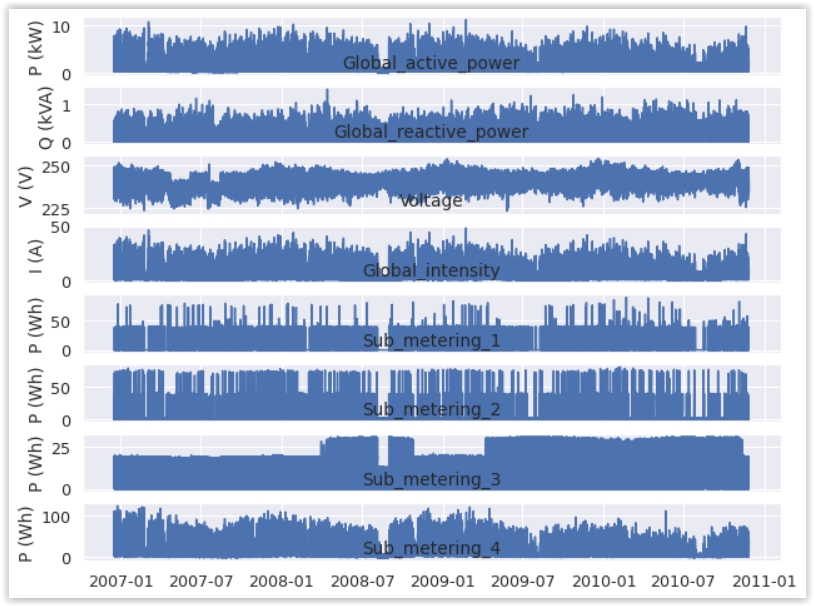
\includegraphics[width=0.99\textwidth]{Figuras/4. Resultados e Discussões/Exer4/Gráfico das variáveis em função do tempo (amostragem por minuto).jpg}
    \caption{Gráfico das variáveis em função do tempo (amostragem por minuto).\\ \textbf{Fonte -} Autores}
    \label{fig: Gráfico das variáveis em função do tempo (amostragem por minuto)}
\end{figure}

Afim de facilitar a visualização desses movimentos periódicos e, conforme discutido na Fundamentação Teórica, foram também realizados os gráficos das variáveis em função do tempo para intervalos horários e diários.

A Figura \ref{fig: Gráfico das variáveis em função do tempo (resampled por hora)} mostra os Gráfico das variáveis em função do tempo (resampled por hora).
\begin{figure}[H]
    \centering
    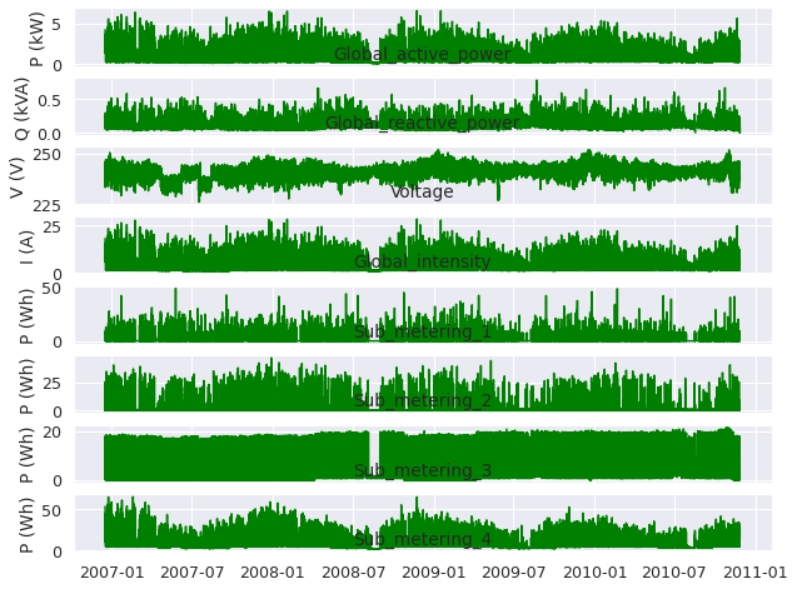
\includegraphics[width=0.99\textwidth]{Figuras/4. Resultados e Discussões/Exer4/Gráfico das variáveis em função do tempo (resampled por hora).jpg}
    \caption{Gráfico das variáveis em função do tempo (resampled por hora).\\ \textbf{Fonte -} Autores}
    \label{fig: Gráfico das variáveis em função do tempo (resampled por hora)}
\end{figure}

A Figura \ref{fig: Gráfico das variáveis em função do tempo (resampled por dia)} mostra os gráficos das variáveis em função do tempo (resampled por dia).
\begin{figure}[H]
    \centering
    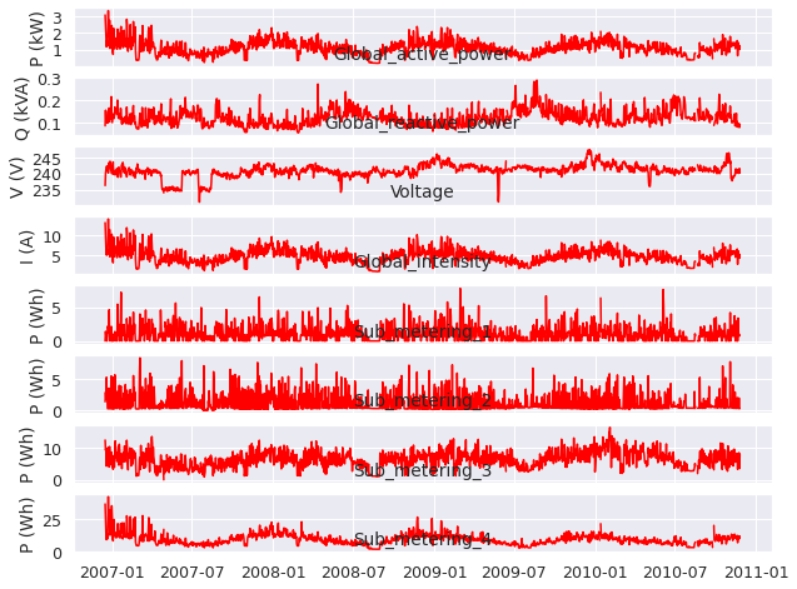
\includegraphics[width=0.99\textwidth]{Figuras/4. Resultados e Discussões/Exer4/Gráfico das variáveis em função do tempo (resampled por dia).jpg}
    \caption{Gráfico das variáveis em função do tempo (resampled por dia).\\ \textbf{Fonte -} Autores}
    \label{fig: Gráfico das variáveis em função do tempo (resampled por dia)}
\end{figure}

O comportamento periódico das variáveis de potência fica ainda mais evidente na Figura \ref{fig: Gráfico das variáveis em função do tempo (resampled por dia)}.

O período de verão ocorre nos meses de julho e agosto. Ocorrem temperaturas mais elevadas nesse período, bem como férias escolares e nas empresas. Se evidencia uma queda na energia elétrica consumida, tanto em termos de potência quando de corrente elétrica. 
Notamente, Sub\_metering\_3, que corresponde ao sistema de climatização (especialmente de aquecimento), e Sub\_metering\_4, que corresponde aos demais aparelhos eletrônicos apresentam queda mais nítida. Essa queda também ocorre para Sub\_metering\_1 e Sub\_metering\_2, embora esses apresentem dados mais "ruidosos" (picos diários importantes).

\subsubsection{Histogramas das variáveis}

Para analisar mais profundamente a tendência de agrupamento de pelo menos parte dos dados, foram plotados os histogramas de cada uma das variáveis. Esses histogramas também podem, em certos casos, fornecer alguma ideia da dependência entre as variáveis. 

A Figura \ref{fig: Histograma das variáveis em função do tempo (amostragem por minuto)} mostra os Histograma das variáveis em função do tempo (amostragem por minuto).
\begin{figure}[H]
    \centering
    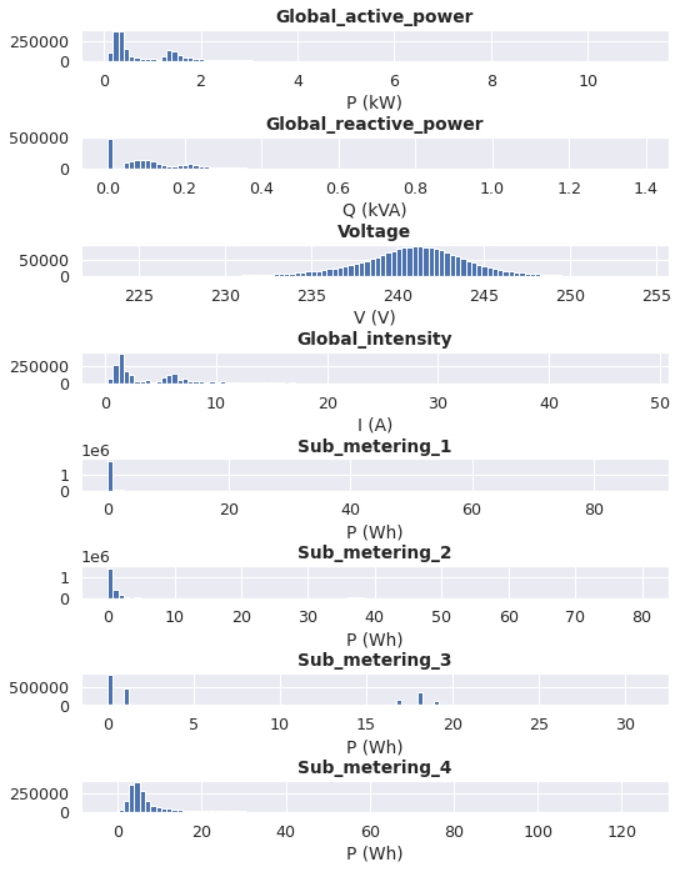
\includegraphics[width=0.99\textwidth]{Figuras/4. Resultados e Discussões/Exer4/Histograma das variáveis em função do tempo (amostragem por minuto).jpg}
    \caption{Histograma das variáveis em função do tempo (amostragem por minuto).\\ \textbf{Fonte -} Autores}
    \label{fig: Histograma das variáveis em função do tempo (amostragem por minuto)}
\end{figure}

Podemos observar uma distribuição bimodal para a potência ativa global, que apresenta dois grupos principais de informação. Há um pico em cerca de $0,3$ kW e um segundo pico notavelmente menor em $1,3$ kW.
Essa distribuição bimodal para a potência ativa global se mantém para o intervalo horário, mas não para o diário, como mostram as Figura \ref{fig: Histograma das variáveis (resampled por hora)} e Figura \ref{fig: Histograma das variáveis (resampled por dia)}.

Na Figura \ref{fig: Histograma das variáveis (resampled por hora)}, esses dois picos que concentram a maior parte dos dados sugerem o uso de dois clusters principais. Pode-se pensar em um terceiro cluster que abrigue os dados da "cauda" \ que se segue ao segundo pico.

Pensando-se em dois clusters principais, uma explicação possível é que o primeiro corresponde a situação em que os moradores da casa estão dormindo ou fora de casa. Nessa situação, o consumo de energia é menor. O segundo pico, menor, corresponde a situação em que luzes, eletrodomésticos e demais aparelhos eletrônicos são utilizados, e corresponde a um maior consumo de energia elétrica.

A Figura \ref{fig: Histograma das variáveis (resampled por hora)} mostra os Histograma das variáveis (resampled por hora).
\begin{figure}[H]
    \centering
    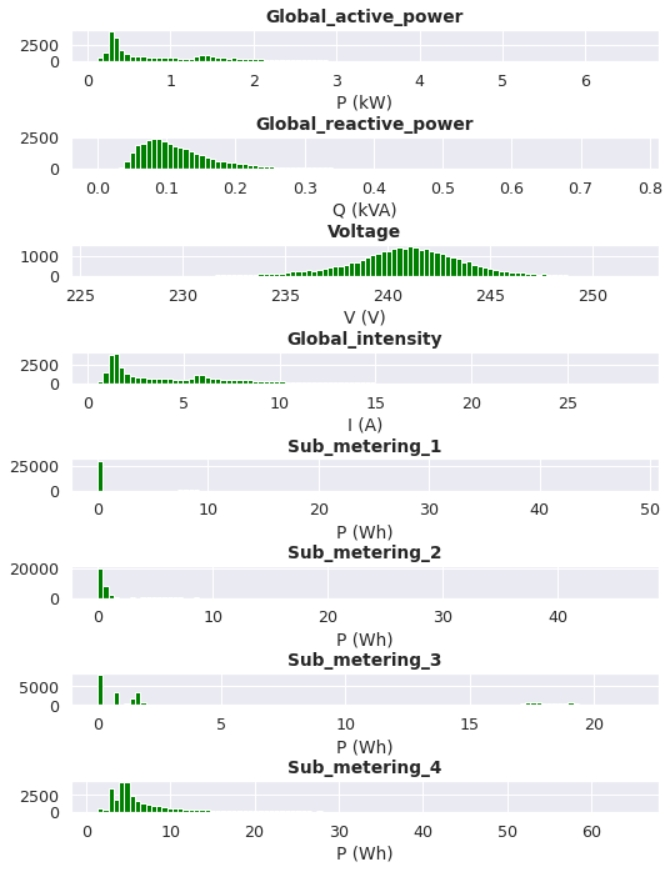
\includegraphics[width=0.99\textwidth]{Figuras/4. Resultados e Discussões/Exer4/Histograma das variáveis (resampled por hora).jpg}
    \caption{Histograma das variáveis (resampled por hora).\\ \textbf{Fonte -} Autores}
    \label{fig: Histograma das variáveis (resampled por hora)}
\end{figure}


A Figura \ref{fig: Histograma das variáveis (resampled por dia)} mostra os Histograma das variáveis (resampled por dia).
\begin{figure}[H]
    \centering
    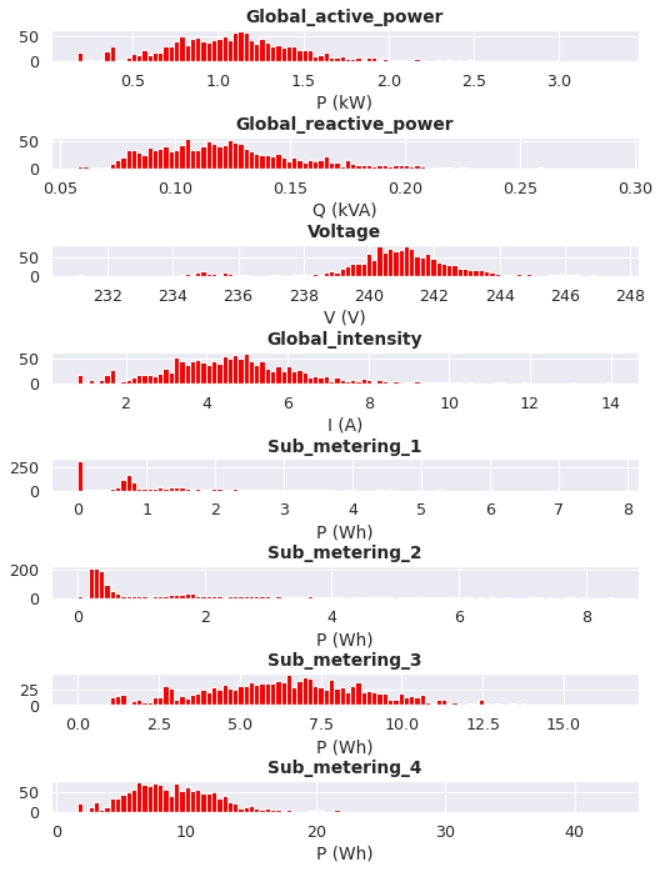
\includegraphics[width=0.99\textwidth]{Figuras/4. Resultados e Discussões/Exer4/Histograma das variáveis (resampled por dia).jpg}
    \caption{Histograma das variáveis (resampled por dia).\\ \textbf{Fonte -} Autores}
    \label{fig: Histograma das variáveis (resampled por dia)}
\end{figure}

Podemos ainda observar uma distribuição da tensão que se aproxima da distribuição gaussiana que mantém-se nos $3$ histogramas.

Também podemos constatar que o comportamento da corrente segue fielmente o comportamento da potência ativa global.

Os medidores Sub\_metering\_1, Sub\_metering\_2 e Sub\_metering\_3, que medem potência ativa (horária), estão obviamente relacionados a potência ativa global.

A fim de melhor compreender a relação dessas variáveis, a correlação entre elas é discutida a seguir.

\subsubsection{Correlação entre as variáveis}

A Figura \ref{fig: Correlaçao entre as variáveis (amostragem por minuto)} mostra as correlações entre as variáveis (amostragem por minuto).
\begin{figure}[H]
    \centering
    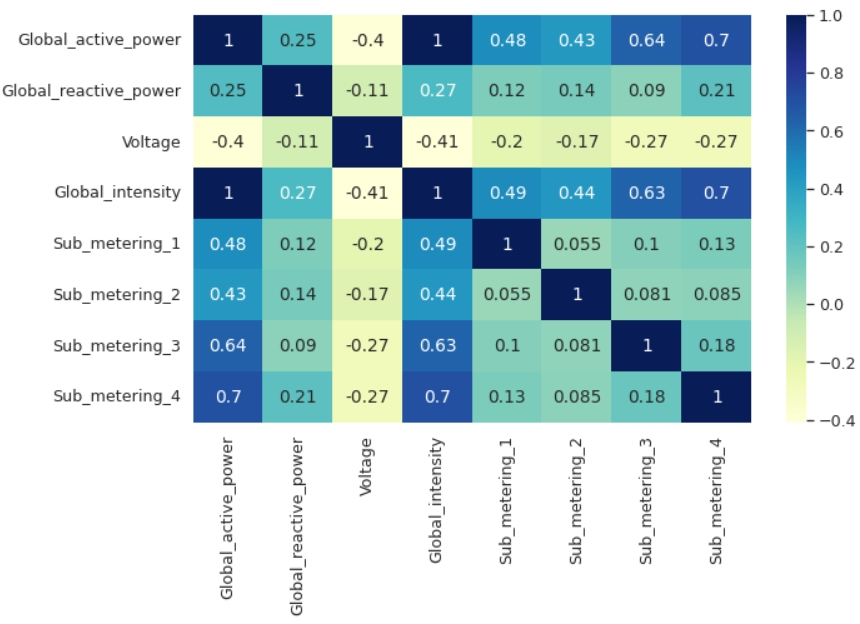
\includegraphics[width=0.80\textwidth]{Figuras/4. Resultados e Discussões/Exer4/Correlaçao entre as variáveis (amostragem por minuto).jpg}
    \caption{Correlações entre as variáveis (amostragem por minuto).\\ \textbf{Fonte -} Autores}
    \label{fig: Correlaçao entre as variáveis (amostragem por minuto)}
\end{figure}

A Figura \ref{fig: Correlaçao entre as variáveis (amostragem por minuto)}, bem como a Figura \ref{fig: Correlação entre as variáveis (resampled por hora)}, evidenciam algumas das constatações anteriores.

A Figura \ref{fig: Correlação entre as variáveis (resampled por hora)} mostra as correlações entre as variáveis (resampled por hora).
\begin{figure}[H]
    \centering
    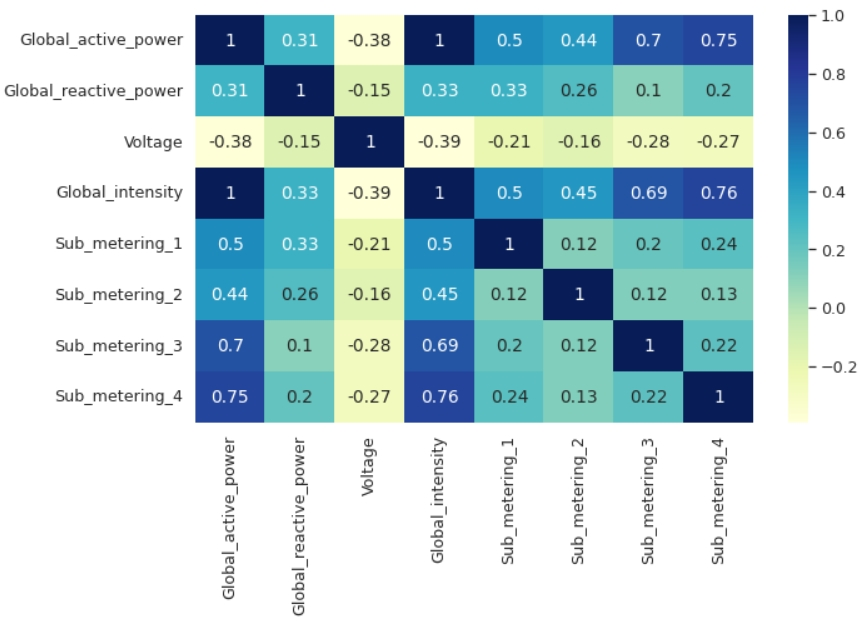
\includegraphics[width=0.80\textwidth]{Figuras/4. Resultados e Discussões/Exer4/Correlação entre as variáveis (resampled por hora).jpg}
    \caption{Correlações entre as variáveis (resampled por hora).\\ \textbf{Fonte -} Autores}
    \label{fig: Correlação entre as variáveis (resampled por hora)}
\end{figure}

A corrente global e a potência ativa globais são totalmente  correlacionadas. Além disso, Sub\_metering\_4 é altamente correlacionadas com ambas. Isso era esperado, uma vez que Sub\_metering\_4 é uma combinação linear da potência ativa global com os outros $3$ medidores.

Esse quarto medidor, sabidamente correlacionado, também serve de parameetro para julgar o que é uma alta correlação nesta aplicação. O terceiro medidor possui valor similar de correlação com a potência global. Os outros dois medidores, um pouco abaixo, ainda apresentam uma correlação significativa com a potência ativa global.

A Figura \ref{fig: Correlação entre as variáveis (resampled por dia)} mostra as correlações entre as variáveis (resampled por dia).
\begin{figure}[H]
    \centering
    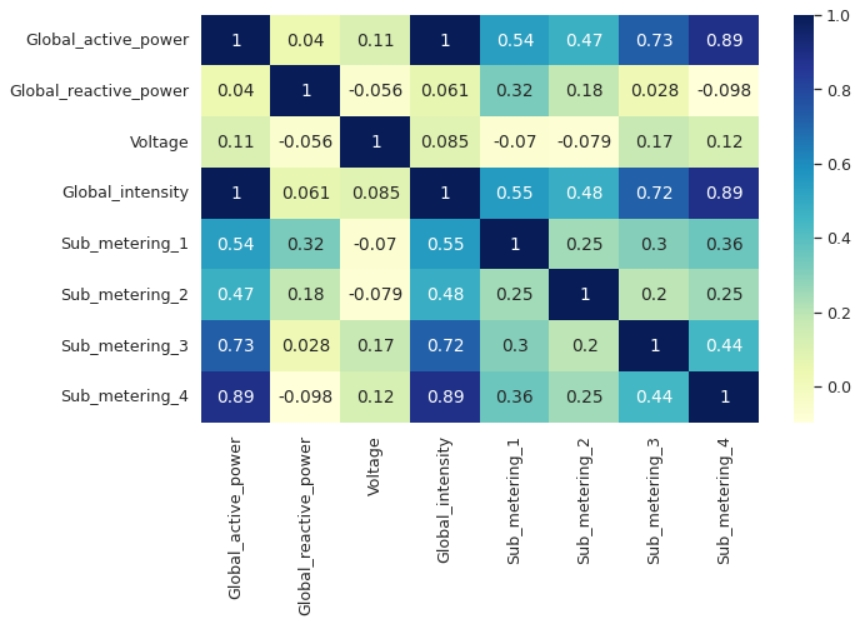
\includegraphics[width=0.80\textwidth]{Figuras/4. Resultados e Discussões/Exer4/Correlação entre as variáveis (resampled por dia).jpg}
    \caption{Correlações entre as variáveis (resampled por dia).\\ \textbf{Fonte -} Autores}
    \label{fig: Correlação entre as variáveis (resampled por dia)}
\end{figure}

Fica evidenciado que este novo intervalo de tempo altera as relações entre as variáveis, já que certas tendências de alta frequência dos dados foram filtradas, como já estava indicado nas etapas anteriores.

Desta forma, baseado nas correlações da Figura \ref{fig: Correlaçao entre as variáveis (resampled por hora)} e nos histogramas, são selecionadas as variáveis Global\_active\_power, Global\_reactive\_power e Voltage, que são menos correlacionadas. Isso evita redundâncias nas informações passados para os modelos de aprendizado, reduzindo o tempo de processamento (o custo computacional), sem perdas expressivas de informação para confirmar a hipótese de dois clusters principais para o consumo de energia.

\subsubsection{Visualização das variáveis selecionadas normalizadas}

A Figura \ref{fig: Visualização das variáveis selecionadas normalizadas} mostra a Visualização das variáveis selecionadas normalizadas.
\begin{figure}[H]
    \centering
    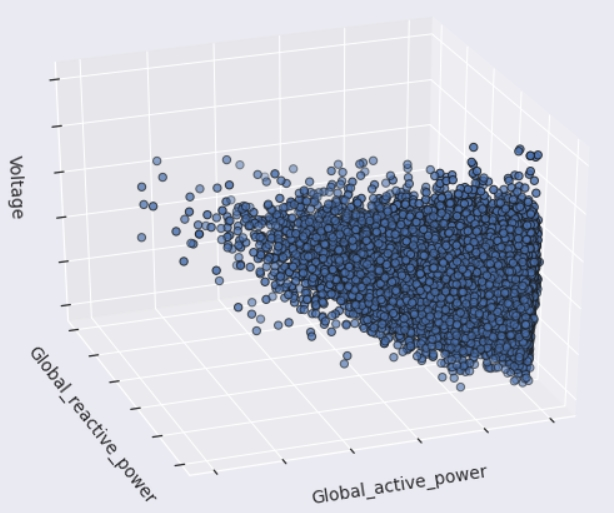
\includegraphics[width=0.90\textwidth]{Figuras/4. Resultados e Discussões/Exer4/Visualização das variáveis selecionadas normalizadas.jpg}
    \caption{Visualização das variáveis selecionadas normalizadas.\\ \textbf{Fonte -} Autores}
    \label{fig: Visualização das variáveis selecionadas normalizadas}
\end{figure}



\subsubsection{Curva do Cotovelo e Coeficiente de Silhueta para k-means}

A Figura \ref{fig: Curva do Cotovelo - Soma dos quadrados versus valores de k para k-means} mostra a Curva do Cotovelo - Soma dos quadrados versus valores de $k$ para k-means, enquanto a Figura \ref{fig: Coeficientes de Silhueta - Coeficientes de Silhueta versus valores de k para k-means} mostra os Coeficientes de Silhueta - Coeficientes de Silhueta versus valores de $k$ para k-means.

\begin{figure}[H]
    \centering
    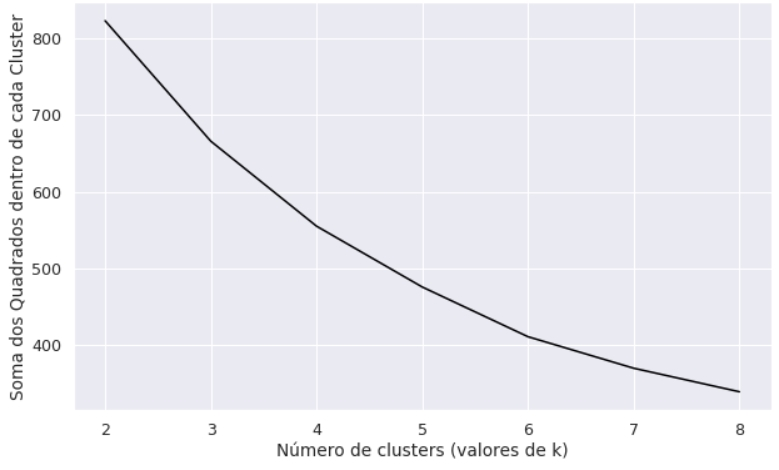
\includegraphics[width=0.80\textwidth]{Figuras/4. Resultados e Discussões/Exer4/Curva do Cotovelo - Soma dos quadrados versus valores de k para k-means.jpg}
    \caption{Curva do Cotovelo - Soma dos quadrados versus valores de k para k-means.\\ \textbf{Fonte -} Autores}
    \label{fig: Curva do Cotovelo - Soma dos quadrados versus valores de k para k-means}
\end{figure}

\begin{figure}[H]
    \centering
    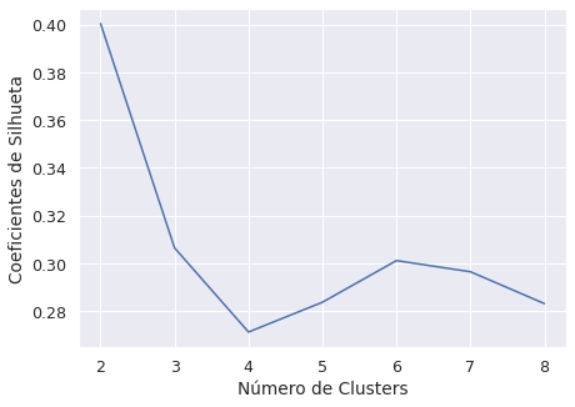
\includegraphics[width=0.80\textwidth]{Figuras/4. Resultados e Discussões/Exer4/Coeficientes de Silhueta - Coeficientes de Silhueta versus valores de k para k-means.jpg}
    \caption{Coeficientes de Silhueta - Coeficientes de Silhueta versus valores de k para k-means.\\ \textbf{Fonte -} Autores}
    \label{fig: Coeficientes de Silhueta - Coeficientes de Silhueta versus valores de k para k-means}
\end{figure}

A Tabela \ref{tab: metricas-k-means} sintetiza as informações numéricas da Figura \ref{fig: Curva do Cotovelo - Soma dos quadrados versus valores de k para k-means} e da Figura \ref{fig: Coeficientes de Silhueta - Coeficientes de Silhueta versus valores de k para k-means}.

\begin{table}[H]
\centering
\begin{tabular}{ccc}
\hline
\textbf{k} & \textbf{\begin{tabular}[c]{@{}c@{}}Métrica de dispersão \\ (Within Cluster Sum of Squares, WCSS)\end{tabular}} & \textbf{Coeficientes de Silhueta} \\ \hline
2          & 822.7057450368584                                                                                              & 0.40049021394565676               \\
3          & 665.8354678854887                                                                                              & 0.3065077452286447                \\
4          & 555.2209768078167                                                                                              & 0.27124295553519806               \\
5          & 475.9829051120406                                                                                              & 0.28373590877014304               \\
6          & 411.267520027729                                                                                               & 0.301171450953407                 \\
7          & 370.21976873821336                                                                                             & 0.2964859717538239                \\
8          & 339.556489822066                                                                                               & 0.28315112572778456               \\ \hline
\end{tabular}
\caption{K-Means: Métrica de dispersão (Within Cluster Sum of Squares, WCSS) e Coeficientes de Silhueta para diferentes valores de k.\\ \textbf{Fonte -} Autores.
}
\label{tab: metricas-k-means}
\end{table}

O valor de $k$ ótimo, em termos do coeficiente de silhueta, é  $2$. Esse não é o valor que reduz mais a dispersão dos dados (o que se reflete no coeficiente $a$ do coeficiente de silhueta), mas aumenta o o coeficiente $b$ do coeficiente de silhueta.

\subsubsection{Visualização das variáveis selecionadas normalizadas - Cluster k-means k = 2}

A Figura \ref{fig: Visualização das variáveis selecionadas normalizadas - Cluster K-means k = 2} mostra os Visualização das variáveis selecionadas normalizadas - Cluster K-means k = 2.
\begin{figure}[H]
    \centering
    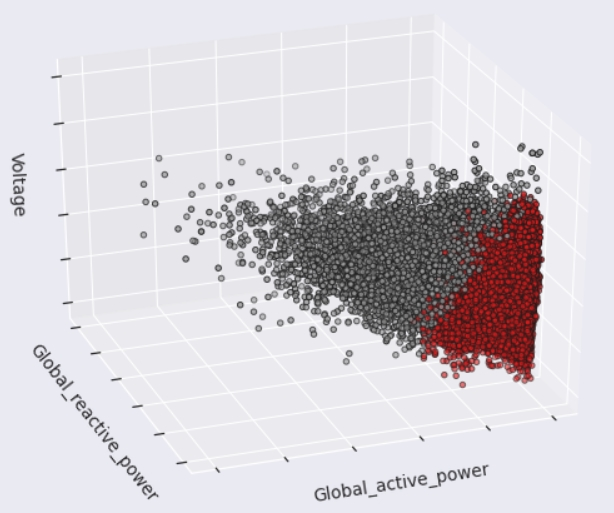
\includegraphics[width=0.99\textwidth]{Figuras/4. Resultados e Discussões/Exer4/Visualização das variáveis selecionadas normalizadas - Cluster K-means k = 2.jpg}
    \caption{Visualização das variáveis selecionadas normalizadas - Cluster K-means k = 2.\\ \textbf{Fonte -} Autores}
    \label{fig: Visualização das variáveis selecionadas normalizadas - Cluster K-means k = 2}
\end{figure}

Centroids:

[[0.07355204 0.14272896 0.61582265]

 [0.30853053 0.19491728 0.49280387]]


\subsubsection{Visualização das variáveis selecionadas normalizadas - Cluster k-means k = 3}

A Figura \ref{fig: Visualização das variáveis selecionadas normalizadas - Cluster K-means k = 3} mostra os Visualização das variáveis selecionadas normalizadas - Cluster K-means k = 3.
\begin{figure}[H]
    \centering
    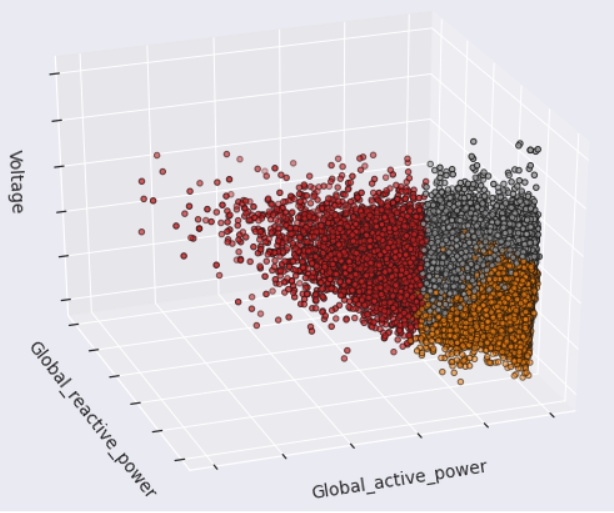
\includegraphics[width=0.90\textwidth]{Figuras/4. Resultados e Discussões/Exer4/Visualização das variáveis selecionadas normalizadas - Cluster K-means k = 3.jpg}
    \caption{Visualização das variáveis selecionadas normalizadas - Cluster K-means k = 3.\\ \textbf{Fonte -} Autores}
    \label{fig: Visualização das variáveis selecionadas normalizadas - Cluster K-means k = 3}
\end{figure}

Centroids: 

[[0.40196201 0.24539978 0.49586753]

 [0.06343258 0.14472396 0.64727527]
 
 [0.17563904 0.1447392  0.49571597]]

\subsubsection{Visualização das variáveis selecionadas normalizadas - Cluster k-means k = 6}

A Figura \ref{fig: Visualização das variáveis selecionadas normalizadas - Cluster K-means k = 6} mostra os Visualização das variáveis selecionadas normalizadas - Cluster K-means k = 6.
\begin{figure}[H]
    \centering
    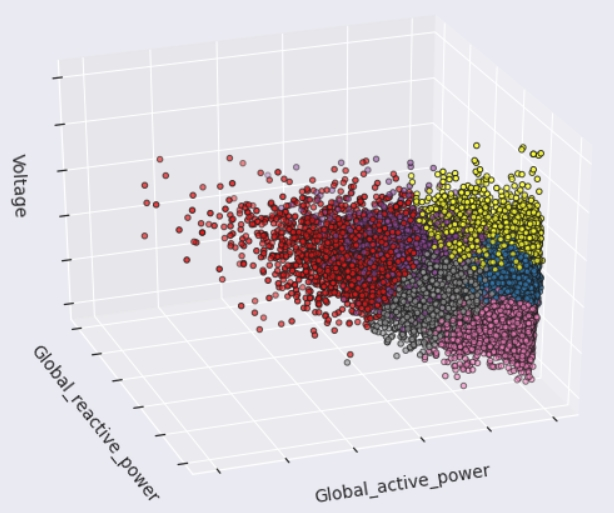
\includegraphics[width=0.99\textwidth]{Figuras/4. Resultados e Discussões/Exer4/Visualização das variáveis selecionadas normalizadas - Cluster K-means k = 6.jpg}
    \caption{Visualização das variáveis selecionadas normalizadas - Cluster K-means k = 6.\\ \textbf{Fonte -} Autores}
    \label{fig: Visualização das variáveis selecionadas normalizadas - Cluster K-means k = 6}
\end{figure}

% Centroids: 

% [[0.47746684 0.23377643 0.44519599]

%  [0.05119687 0.15323246 0.58498542]
 
%  [0.23615379 0.35105636 0.55220657]
 
%  [0.11839841 0.12823863 0.37684934]
 
%  [0.06804891 0.1216586  0.72600341]
 
%  [0.24790082 0.1320107  0.5596597 ]]

Pode-se observar que o aumento do número de cluster tende a preservar parte do cluster à esquerda nas imagens e dividir os clusters mais a direita.

\subsubsection{Classificação com K-NN}

A Figura \ref{fig: Erro de classificação incorreta versus k pada 2 classes determinadas por k-means} mostra os Erro de classificação incorreta versus k pada 2 classes determinadas por k-means.
\begin{figure}[H]
    \centering
    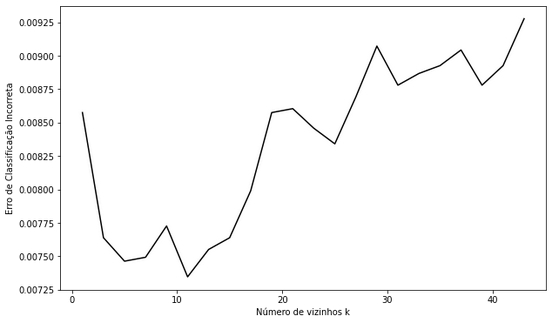
\includegraphics[width=0.99\textwidth]{Figuras/4. Resultados e Discussões/Exer4/Erro de classificação incorreta versus k pada 2 classes determinadas por k-means.jpg}
    \caption{Erro de classificação incorreta versus k pada 2 classes determinadas por k-means.\\ \textbf{Fonte -} Autor}
    \label{fig: Erro de classificação incorreta versus k pada 2 classes determinadas por k-means}
\end{figure}

O número de vizinhos ótimo foi obtido para $k = 11$, com $\text{Mean Accuracy} = 0,993$ e $\text{min(MSE)} = 0.00734$ para duas classes.

A Figura \ref{fig: Erro de classificação incorreta versus k para 3 classes determinadas por k-means} mostra os Erro de classificação incorreta versus k para 3 classes determinadas por k-means.
\begin{figure}[H]
    \centering
    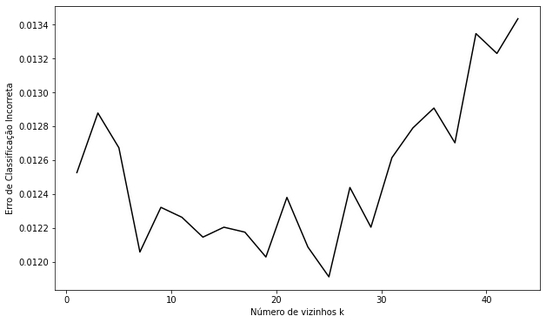
\includegraphics[width=0.99\textwidth]{Figuras/4. Resultados e Discussões/Exer4/Erro de classificação incorreta versus k para 3 classes determinadas por k-means.jpg}
    \caption{Erro de classificação incorreta versus k para 3 classes determinadas por k-means.\\ \textbf{Fonte -} Autor}
    \label{fig: Erro de classificação incorreta versus k para 3 classes determinadas por k-means}
\end{figure}

% 0 número de vizinhos ótimo é: 25 Mean Accuracy 0.9880882215866528 min(MSE) = 0.01191177841334723
O número de vizinhos ótimo foi obtido para $k = 25$, com $\text{Mean Accuracy} = 0,9881$ e $\text{min(MSE)} = 0.01191$ para $3$ classes.


A Figura \ref{fig: Erro de classificação incorreta versus k para 6 classes determinadas por k-means} mostra os Erro de classificação incorreta versus k para 6 classes determinadas por k-means.
\begin{figure}[H]
    \centering
    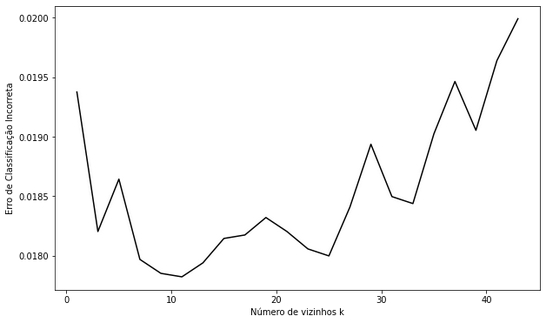
\includegraphics[width=0.99\textwidth]{Figuras/4. Resultados e Discussões/Exer4/Erro de classificação incorreta versus k para 6 classes determinadas por k-means.jpg}
    \caption{Erro de classificação incorreta versus k para 6 classes determinadas por k-means.\\ \textbf{Fonte -} Autor}
    \label{fig: Erro de classificação incorreta versus k para 6 classes determinadas por k-means}
\end{figure}

% 0 número de vizinhos ótimo é: 11 Mean Accuracy 0.9821761491481839 min(MSE) = 0.017823850851816148
O número de vizinhos ótimo foi obtido para $k = 11$, com $\text{Mean Accuracy} = 0,9821$ e $\text{min(MSE)} = 0.01782$ para $6$ classes.

Dessa forma, se fornece mais uma evidência para a utilização de um menor número de classes: o número de $k$ vizinhos ótimo mínimo é obtido para $2$ e $6$, o que reduz a carga computacional. As vantagens da utilização de $k = 2$ para o coeficiente de silhueta reforçam essa escolha.  

\subsection{Exercício 11}
 
Uma primeira constatação é que o algoritmo k-medoids (PAM) necessitou de um tempo significativamente maior de computação que o algoritmo k-means na plataforma Colab com as versões dos módulos utilizados. Para gerar a Curva do Cotovelo e do Coeficiente de Silhueta, foram necessários 2 h 32 min e 41 s (sendo cerca de 2 minutos para $k = 2$, 8 minutos para $k = 3$, 15 minutos para $k = 4$ e 25 minutos para $k = 5$, por exemplo).
 
\subsubsection{Curva do Cotovelo e Coeficiente de Silhueta para k-medoids (PAM)}
 
 A Figura \ref{fig: Curva do Cotovelo - Soma dos quadrados versus valores de k para PAM k-medoids} mostra os Curva do Cotovelo - Soma dos quadrados versus valores de k para PAM k-medoids.
\begin{figure}[H]
    \centering
    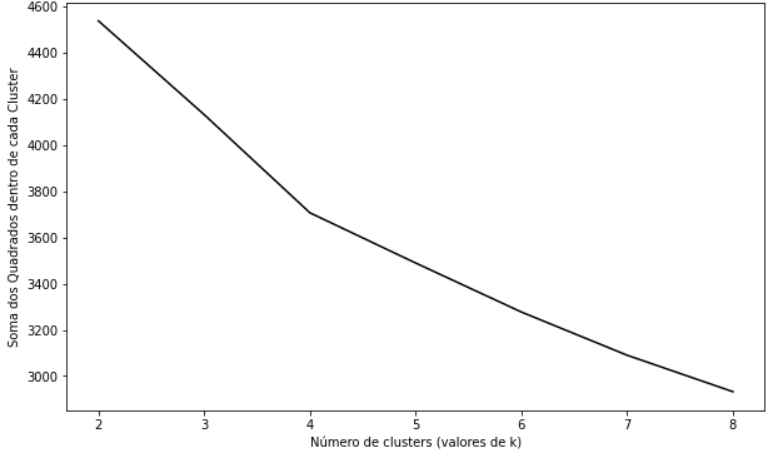
\includegraphics[width=0.99\textwidth]{Figuras/4. Resultados e Discussões/Exer4/Curva do Cotovelo - Soma dos quadrados versus valores de k para PAM k-medoids.jpg}
    \caption{Curva do Cotovelo - Soma dos quadrados versus valores de k para PAM k-medoids.\\ \textbf{Fonte -} Autores}
    \label{fig: Curva do Cotovelo - Soma dos quadrados versus valores de k para PAM k-medoids}
\end{figure}

A Figura \ref{fig: Coeficientes de Silhueta - Coeficientes de Silhueta versus valores de k para PAM k-medoids} mostra os Coeficientes de Silhueta - Coeficientes de Silhueta versus valores de k para PAM k-medoids.
\begin{figure}[H]
    \centering
    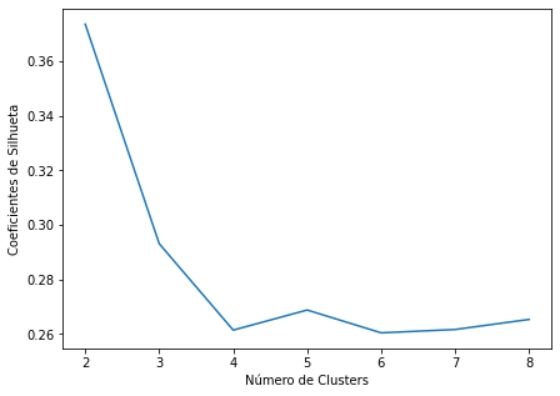
\includegraphics[width=0.99\textwidth]{Figuras/4. Resultados e Discussões/Exer4/Coeficientes de Silhueta - Coeficientes de Silhueta versus valores de k para PAM k-medoids.jpg}
    \caption{Coeficientes de Silhueta - Coeficientes de Silhueta versus valores de k para PAM k-medoids.\\ \textbf{Fonte -} Autores}
    \label{fig: Coeficientes de Silhueta - Coeficientes de Silhueta versus valores de k para PAM k-medoids}
\end{figure}

A Tabela \ref{tab: metricas-k-medoids} sintetiza as informações numéricas da Figura \ref{fig: Curva do Cotovelo - Soma dos quadrados versus valores de k para PAM k-medoids} e da Figura \ref{fig: Coeficientes de Silhueta - Coeficientes de Silhueta versus valores de k para PAM k-medoids}.
 
\begin{table}[H]
\centering
\begin{tabular}{ccc}
\hline
\textbf{k} & \textbf{\begin{tabular}[c]{@{}c@{}}Métrica de dispersão \\ (Within Cluster Sum of Squares, WCSS)\end{tabular}} & \textbf{Coeficientes de Silhueta} \\ \hline
2          & 4536.521734745653                                                                                              & 0.37362479819592515               \\
3          & 4130.9698995473                                                                                                & 0.29309845549796026               \\
4          & 3706.228876626484                                                                                              & 0.2614015795146218                \\
5          & 3488.9812810363164                                                                                             & 0.2687737999210143                \\
6          & 3276.9518201949168                                                                                             & 0.26039828351782524               \\
7          & 3090.0707409641996                                                                                             & 0.2616294450608593                \\
8          & 2932.403180249776                                                                                              & 0.26531918644281965                             \\ \hline
\end{tabular}
\caption{K-Medoids: Métrica de dispersão (Within Cluster Sum of Squares, WCSS) e Coeficientes de Silhueta para diferentes valores de k.\\ \textbf{Fonte -} Autores.}
\label{tab: metricas-k-medoids}
\end{table}

O valor de $K$ ótimo, em termos do coeficiente de silhueta, é também aqui $2$.

Os valores de coeficiente de silhueta são similares, indicando, em conjunto com a métrica de dispersão, que o algoritmo não aumentou a coesão e separação dos clusters neste problema. Considerando este fato e o tempo de processamento substancialmente maior, o algoritmo k-means se mostra preferivel.

\subsubsection{Visualização das variáveis selecionadas normalizadas - Cluster PAM k-medoids k = 2}

A Figura \ref{fig: Visualização das variáveis selecionadas normalizadas - Cluster PAM K-medoids k = 2} mostra os Visualização das variáveis selecionadas normalizadas - Cluster PAM K-medoids k = 2.
\begin{figure}[H]
    \centering
    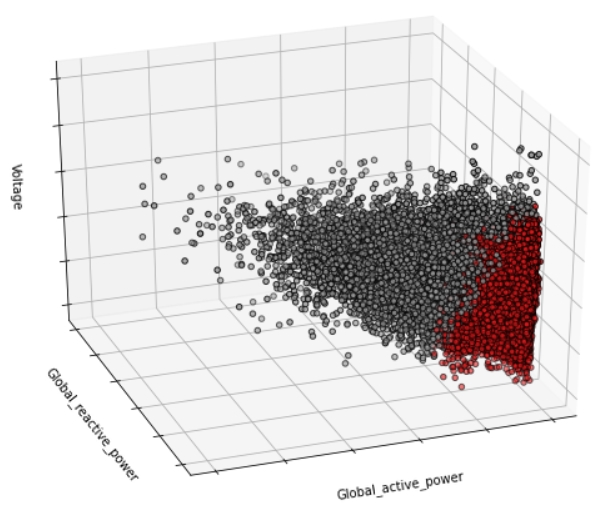
\includegraphics[width=0.99\textwidth]{Figuras/4. Resultados e Discussões/Exer4/Visualização das variáveis selecionadas normalizadas - Cluster PAM K-medoids k = 2.jpg}
    \caption{Visualização das variáveis selecionadas normalizadas - Cluster PAM K-medoids k = 2.\\ \textbf{Fonte -} Autores}
    \label{fig: Visualização das variáveis selecionadas normalizadas - Cluster PAM K-medoids k = 2}
\end{figure}
 
Centroids: 

[[0.04949352 0.1397331  0.62384834]

[0.25716742 0.16457167 0.52808414]]
 
\subsubsection{Visualização das variáveis selecionadas normalizadas - Cluster PAM k-medoids k = 3}
 
 A Figura \ref{fig: Visualização das variáveis selecionadas normalizadas - Cluster PAM K-medoids k = 3} mostra os Visualização das variáveis selecionadas normalizadas - Cluster PAM K-medoids k = 3.
\begin{figure}[H]
    \centering
    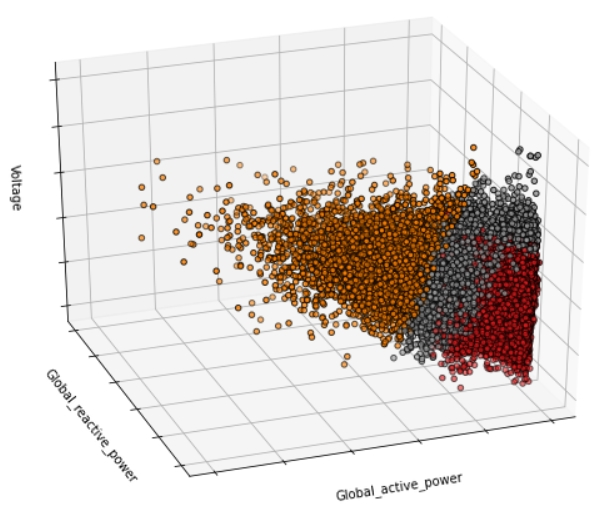
\includegraphics[width=0.99\textwidth]{Figuras/4. Resultados e Discussões/Exer4/Visualização das variáveis selecionadas normalizadas - Cluster PAM K-medoids k = 3.jpg}
    \caption{Visualização das variáveis selecionadas normalizadas - Cluster PAM K-medoids k = 3.\\ \textbf{Fonte -} Autores}
    \label{fig: Visualização das variáveis selecionadas normalizadas - Cluster PAM K-medoids k = 3}
\end{figure}

Centroids:

[[0.04540747 0.14244511 0.62616285]

 [0.37316672 0.20985794 0.48773377]
 
 [0.19362908 0.13607404 0.54338416]]

\subsubsection{Visualização das variáveis selecionadas normalizadas - Cluster PAM k-medoids k = 3}

A Figura \ref{fig: Visualização das variáveis selecionadas normalizadas - Cluster PAM K-medoids k = 6} mostra os Visualização das variáveis selecionadas normalizadas - Cluster PAM K-medoids k = 6.
\begin{figure}[H]
    \centering
    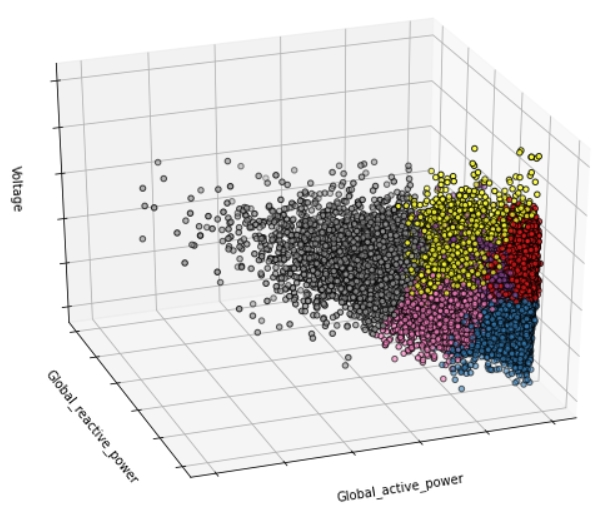
\includegraphics[width=0.99\textwidth]{Figuras/4. Resultados e Discussões/Exer4/Visualização das variáveis selecionadas normalizadas - Cluster PAM K-medoids k = 6.jpg}
    \caption{Visualização das variáveis selecionadas normalizadas - Cluster PAM K-medoids k = 6.\\ \textbf{Fonte -} Autor}
    \label{fig: Visualização das variáveis selecionadas normalizadas - Cluster PAM K-medoids k = 6}
\end{figure}

% Centroids: [[0.03973153 0.12311666 0.55046834]
%  [0.04503459 0.11356005 0.70204277]
%  [0.05484837 0.21545415 0.60845242]
%  [0.2263123  0.13263022 0.46857837]
%  [0.21867361 0.13267327 0.61306224]
%  [0.4067614  0.25570383 0.49197276]]

Pode-se observar que o aumento do número de cluster tende a preservar parte do cluster à esquerda nas imagens e dividir os clusters mais a direita.

\subsubsection{Classificação com K-NN}

A Figura \ref{fig: Erro de classificação incorreta versus k pada 2 classes determinadas por k-medoids} mostra os Erro de classificação incorreta versus k pada 2 classes determinadas por k-medoids.
\begin{figure}[H]
    \centering
    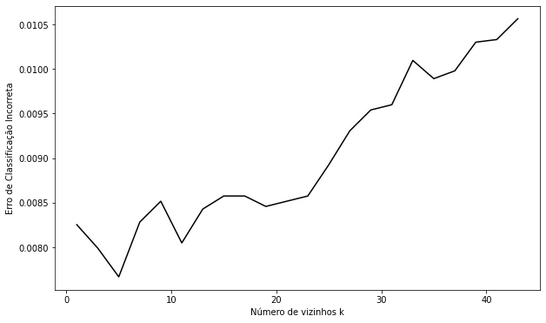
\includegraphics[width=0.99\textwidth]{Figuras/4. Resultados e Discussões/Exer4/Erro de classificação incorreta versus k pada 2 classes determinadas por k-medoids.jpg}
    \caption{Erro de classificação incorreta versus k pada 2 classes determinadas por k-medoids.\\ \textbf{Fonte -} Autor}
    \label{fig: Erro de classificação incorreta versus k pada 2 classes determinadas por k-medoids}
\end{figure}

% 0 número de vizinhos ótimo é: 5 Mean Accuracy 0.9923321212507513 min(MSE) = 0.00766787874924868
0 número de vizinhos ótimo foi obtido para $k = 5$, com $\text{Mean Accuracy} = 0,9923$ e $\text{min(MSE)} = 0.007668$.

A Figura \ref{fig: Erro de classificação incorreta versus k pada 3 classes determinadas por k-medoids} mostra os Erro de classificação incorreta versus k pada 3 classes determinadas por k-medoids.
\begin{figure}[H]
    \centering
    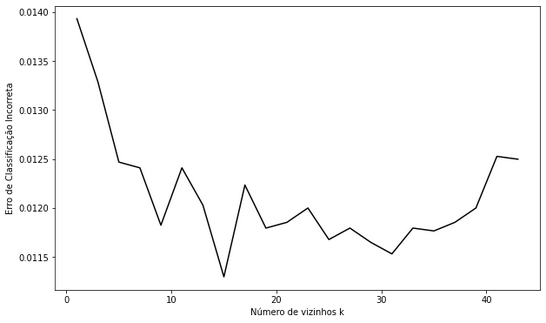
\includegraphics[width=0.99\textwidth]{Figuras/4. Resultados e Discussões/Exer4/Erro de classificação incorreta versus k pada 3 classes determinadas por k-medoids.jpg}
    \caption{Erro de classificação incorreta versus k pada 3 classes determinadas por k-medoids.\\ \textbf{Fonte -} Autor}
    \label{fig: Erro de classificação incorreta versus k pada 3 classes determinadas por k-medoids}
\end{figure}

% 0 número de vizinhos ótimo é: 15 Mean Accuracy 0.9887028728790268 min(MSE) = 0.011297127120973194
0 número de vizinhos ótimo foi obtido para $k = 15$, com $\text{Mean Accuracy} = 0,9887$ e $\text{min(MSE)} = 0.01129$.

Dessa forma, se o método PAM com K-Medoids fosse utilizado, a utilização de duas classes somente com $k = 5$ permite uma menor carga computacional, além de corresponder a configuração com maior coeficiente de silhueta. Esse coeficiente de silhueta não é, no entanto, muito elevado, como indica a dispersão dos dados. Esta é relativamente alta, como mostra a "Curva do cotovelo" ($a$ mais elevado, indicando uma coesão não tão boa).

\subsection{Exercício 12}
Percebe-se ao verificar a documentação \citep{sklearn_kmeans_ref} do método kmeans na biblioteca sklearn percebe-se que há uma preocupação para se performar otimizações. Particularmente, é importante a inicialização dos centroides inicias em locais adequados e plausíveis de serem perto dos locais finais dos centroides. Há um algoritmo denominado k-means++ responsável por essa parte, em vez de se escolher pontos aleatórios pode-se inicializar onde há maior concentração de dados, mantendo certa distância e testar-se alguns centroides iniciais antes de se executar todas as outras iterações.


%%%%%%%%%%%%%%%%%%%%%%%%%%%%%%%%%%%%%%%%%%%% EXERCICIO 15

\subsection{Exercício 15}

Os resultados indicam um resultado bastante satisfatório para quando todas as características geométricas são levadas em consideração, e melhor ainda quando normalizadas conforme apontam o ARI e o \textit{Adjusted Mutual Info} conforme se vê na Tabela 3.
Particularmente no caso de usar apenas as 3 características selecionadas (área, coef. de assimetria e comprimento da fenda) os resultados com as variáveis normalizadas apresentaram métricas piores. Aqui levanta-se a suspeita da qualidade das métricas pois um dos efeitos da normalização é elevar o peso das variáveis de menor desvio padrão ante as de maior desvio padrão. É o caso da comprimento da fenda e do coeficiente de assimetria que apresentam grande sobreposição como se pode ver na figura 8 com desvio padrão relativamente menor. Com a normalização essas duas variáveis tornaram-se mais relevantes, reduzindo o desempenho.

%\begin{table}[H]
    \centering
    \begin{tabular}{c c c} 
        \toprule
        \textbf{Classe} & Área & Perímetro & Compacidade & Comprimento & Largura & Coef. de assimetria & Comp. da fenda\\ [0.5ex] 
        \midrule
        A & 11.856 & 13.248 & 0.848 & 5.232 & 2.849 & 4.742 & 5.102\\
        \hline
        B & 14.437 & 14.337 & 0.882 & 5.515 & 3.259 & 2.707 & 5.121 \\
        \hline
        C & 18.495 & 16.203 & 0.884 & 6.176 & 3.698 & 3.632 & 6.042 \\
        \bottomrule
    \end{tabular}
    \caption{\label{tabela_tabuadas} Centro dos clusters ajustados usando o k-means com variáveis normalizadas \\ \textbf{Fonte -} os Autores.}
\end{table}

\subsubsection{Desempenho}
\begin{table}[H]
    \centering
    \begin{tabular}{c c c} 
        \toprule
        \textbf{Caso} & \textbf{ARI} & \textbf{Ajusted Mutual Info}\\ [0.5ex] 
        \midrule
        Todas as 7 características & 0.716620 & 0.692216 \\
        \hline
        Todas as 7 características, mas normalizadas & 0.77329 & 0.725453 \\
        \hline
        Apenas área, coef. de assimetria e comp. da fenda & 0.713243 & 0.682330 \\
        \hline
        Apenas área, coef. de assimetria e comp. da fenda, normalizados & 0.681486 & 0.656300 \\
        \bottomrule
    \end{tabular}
    \caption{\label{tabela_tabuadas} Métricas de desempenho obtidas para cada um dos conjuntos de clusters. \\ \textbf{Fonte -} os Autores.}
\end{table}

\subsubsection{Matrizes de dispersão}
\begin{figure}[H]
    \centering
    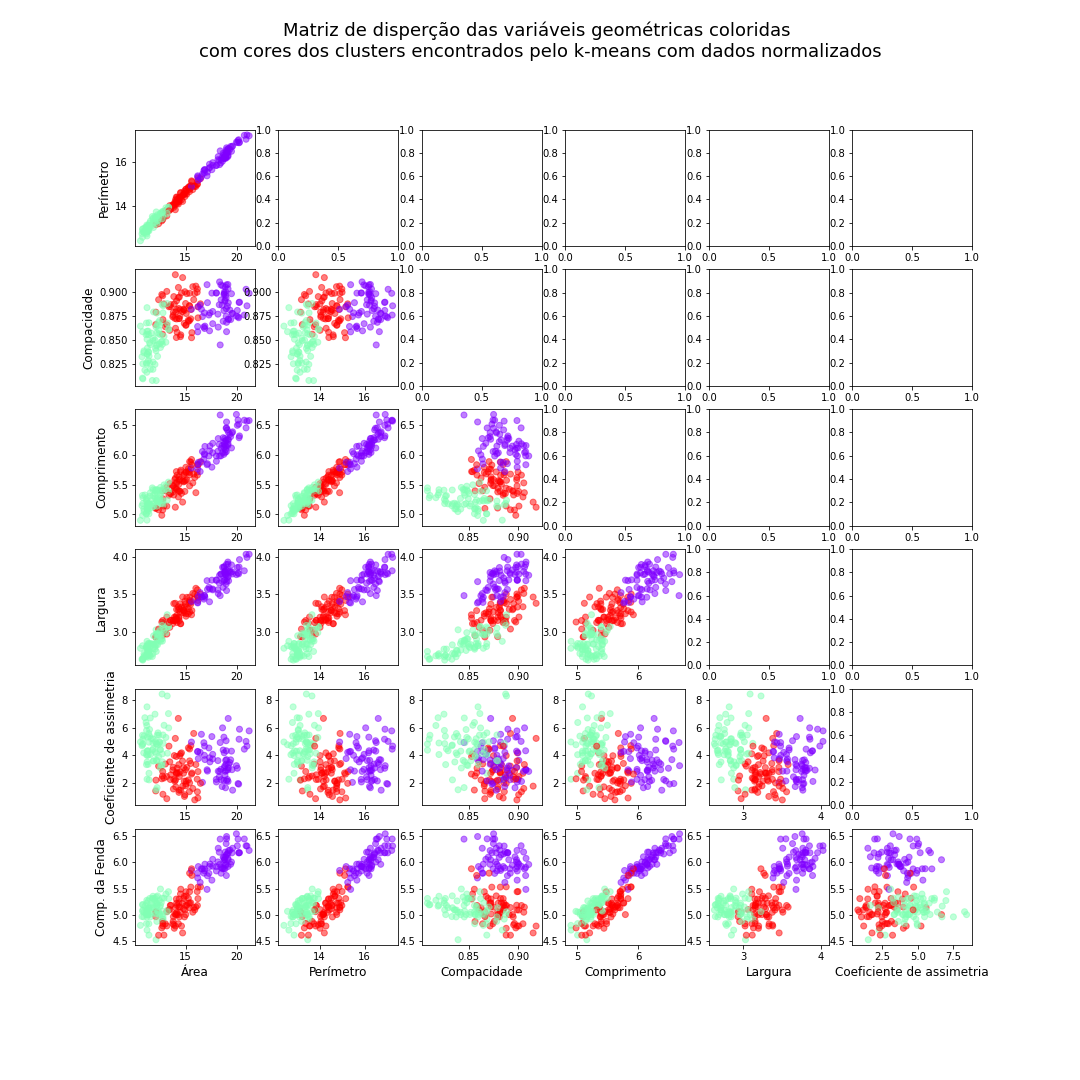
\includegraphics[width=0.99\textwidth]{Figuras/4. Resultados e Discussões/Exer15/fig15b-k-means-normalizado}
    \caption{Matriz de dispersão colorida com clusters gerados a partir dos dados normalizados.\\ \textbf{Fonte -} os Autores}
    \label{fig: Matriz de dispersão colorida com clusters executados a partir dos dados normalizados.}
\end{figure}

\begin{figure}[H]
    \centering
    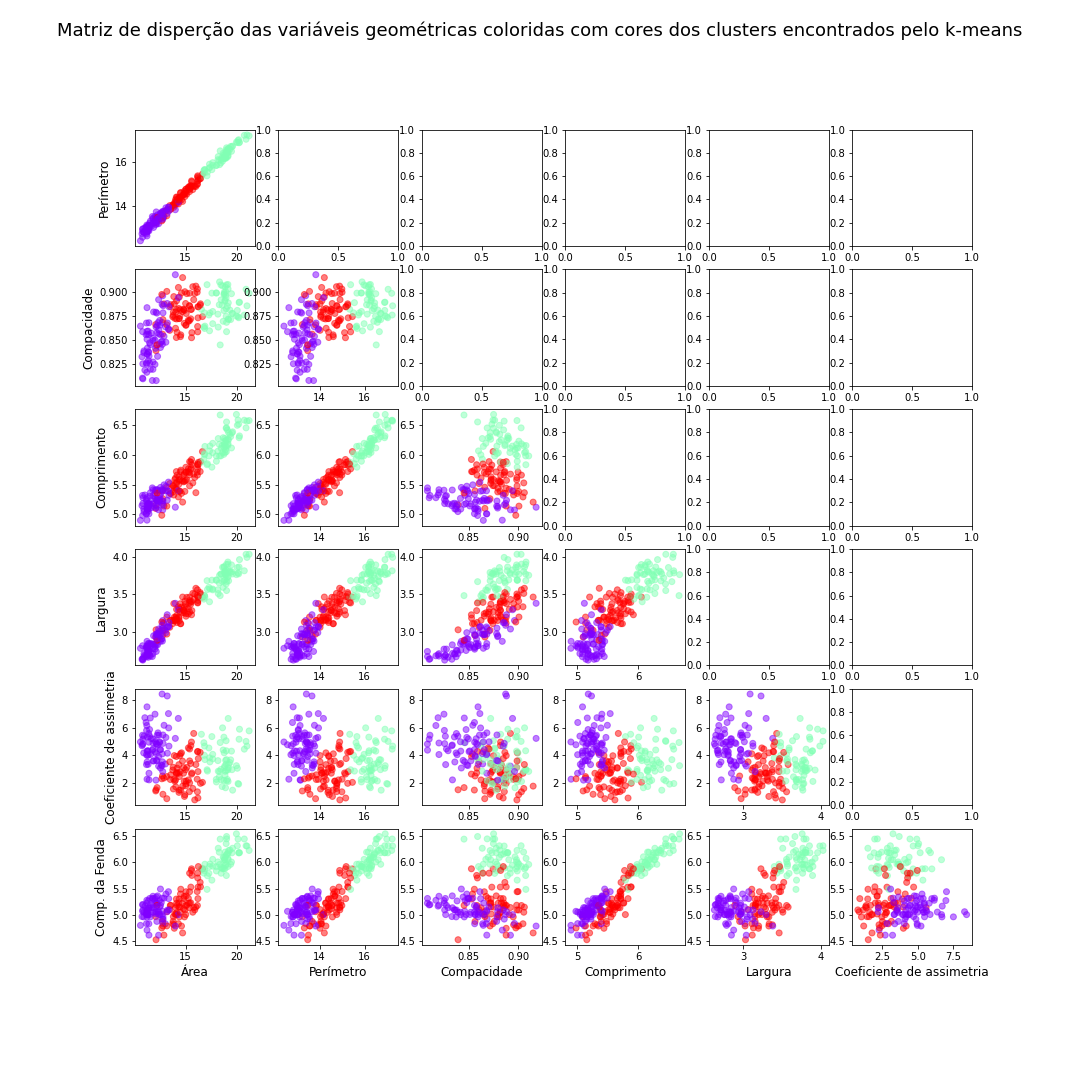
\includegraphics[width=0.99\textwidth]{Figuras/4. Resultados e Discussões/Exer15/fig15b-k-means}
    \caption{Matriz de dispersão colorida com clusters gerados a partir dos dados (sem normalização).\\ \textbf{Fonte -} os Autores}
    \label{fig: Matriz de dispersão colorida com clusters executados a partir dos dados (sem normalização).}
\end{figure}

\begin{figure}[H]
    \centering
    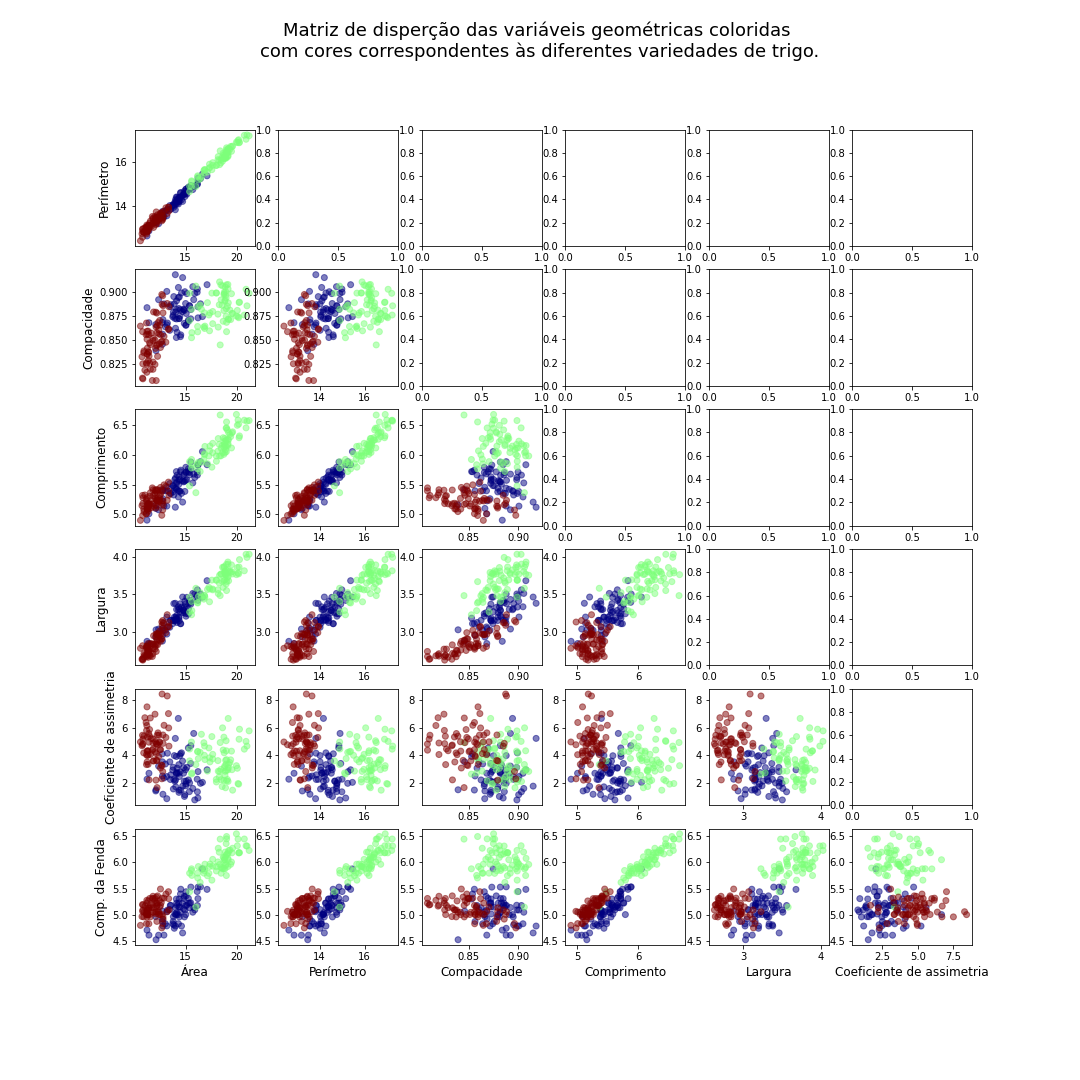
\includegraphics[width=0.99\textwidth]{Figuras/4. Resultados e Discussões/Exer15/fig15b-variedades}
    \caption{Matriz de dispersão colorida por variedade de trigo.\\ \textbf{Fonte -} os Autores}
    \label{fig: Matriz de dispersão colorida por variedade de trigo.}
\end{figure}


\subsection{Exercício 16}
Com a metodologia descrita pode-se plotar as seguintes curvas de somas dos quadrados dos clusters e coeficiente de silhueta médio:

Observa-se que tanto a \textit{WCSS} como a silhueta se reduz com o aumento do valor k, no entanto valores menores de \textit{WCSS} são desejados enquanto valores maiores de coeficiente de silhueta são procurados. Faz-se necessário avaliar o \textit{trade-off} entre as duas situações.


\begin{figure}[H]
    \centering
    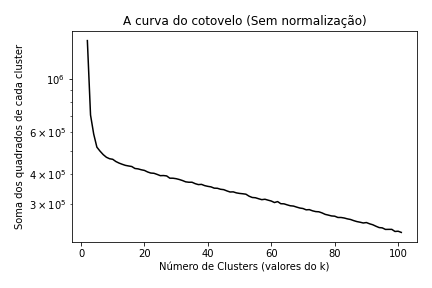
\includegraphics[width=0.7\textwidth]{Figuras/4. Resultados e Discussões/Exer16/fig16A-CurvaCotoveloProdutos2-102.png}
    \caption{Curva WCSS para valores não normalizados\\ \textbf{Fonte -} os Autores}
    \label{fig: fig16A-CurvaCotoveloProdutos2-102.png}
\end{figure}

\begin{figure}[H]
    \centering
    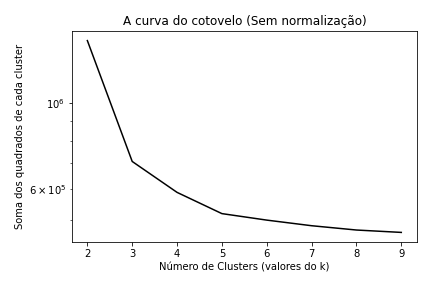
\includegraphics[width=0.75\textwidth]{Figuras/4. Resultados e Discussões/Exer16/fig16A-CurvaCotoveloProdutos2-10.png}
    \caption{Curva WCSS ampliada para valores não normalizados\\ \textbf{Fonte -} os Autores}
    \label{fig: fig16A-CurvaCotoveloProdutos2-10.png}
\end{figure}

\begin{figure}[H]
    \centering
    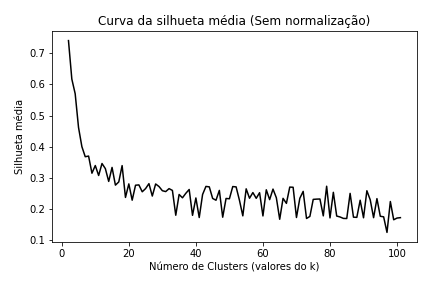
\includegraphics[width=0.75\textwidth]{Figuras/4. Resultados e Discussões/Exer16/fig16A-SilhuetaProdutos2-102.png}
    \caption{Curva Silhueta para valores não normalizados\\ \textbf{Fonte -} os Autores}
    \label{fig: fig16A-SilhuetaProdutos2-102.png}
\end{figure}

\begin{figure}[H]
    \centering
    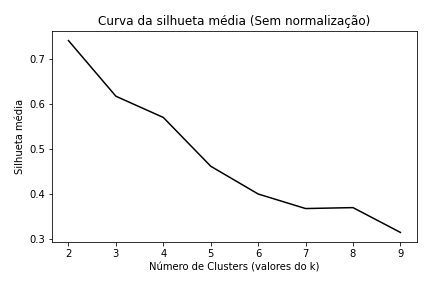
\includegraphics[width=0.75\textwidth]{Figuras/4. Resultados e Discussões/Exer16/fig16A-SilhuetaProdutos2-10.png}
    \caption{Curva Silhueta ampliada para valores não normalizados\\ \textbf{Fonte -} os Autores}
    \label{fig: fig16A-SilhuetaProdutos2-10.png}
\end{figure}

%%%%%%%%%% GRAFICOS EXERCICIO 16 NORMALIZADO

\begin{figure}[H]
    \centering
    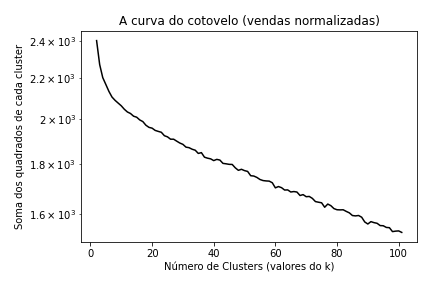
\includegraphics[width=0.75\textwidth]{Figuras/4. Resultados e Discussões/Exer16/fig16B-CurvaCotoveloProdutos2-102.png}
    \caption{Curva WCSS para valores normalizados\\ \textbf{Fonte -} os Autores}
    \label{fig: Matriz de dispersão colorida por variedade de trigo.}
\end{figure}

\begin{figure}[H]
    \centering
    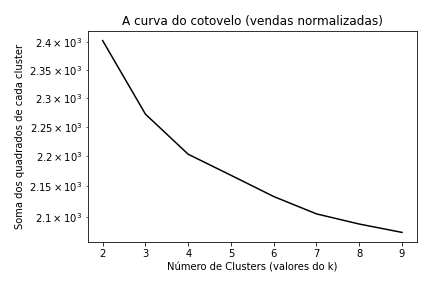
\includegraphics[width=0.75\textwidth]{Figuras/4. Resultados e Discussões/Exer16/fig16B-CurvaCotoveloProdutos2-10.png}
    \caption{Curva WCSS ampliada para para valores normalizados\\ \textbf{Fonte -} os Autores}
    \label{fig: Matriz de dispersão colorida por variedade de trigo.}
\end{figure}

\begin{figure}[H]
    \centering
    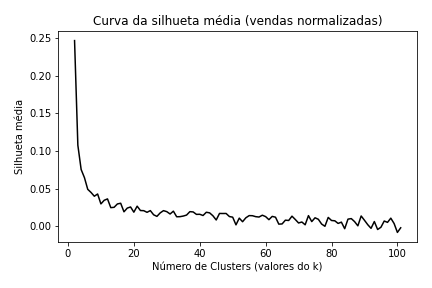
\includegraphics[width=0.75\textwidth]{Figuras/4. Resultados e Discussões/Exer16/fig16B-SilhuetaProdutos2-102.png}
    \caption{Curva Silhueta para valores normalizados\\ \textbf{Fonte -} os Autores}
    \label{fig: Matriz de dispersão colorida por variedade de trigo.}
\end{figure}

\begin{figure}[H]
    \centering
    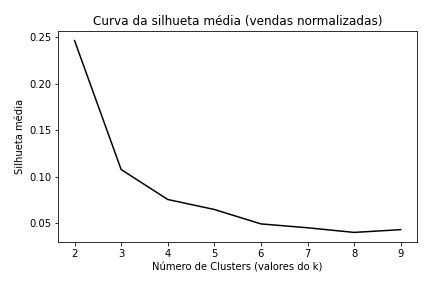
\includegraphics[width=0.75\textwidth]{Figuras/4. Resultados e Discussões/Exer16/fig16B-SilhuetaProdutos2-10.png}
    \caption{Curva Silhueta ampliada para valores normalizados\\ \textbf{Fonte -} os Autores}
    \label{fig: Matriz de dispersão colorida por variedade de trigo.}
\end{figure}